\begin{figure*}[t]
\centering
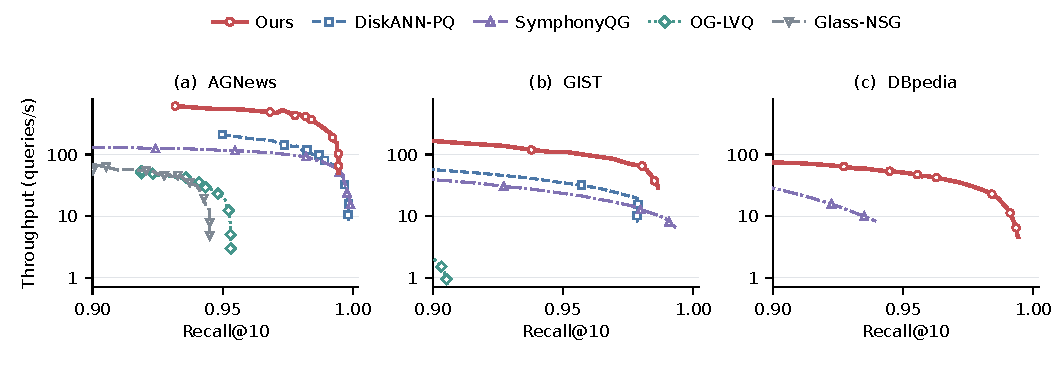
\includegraphics[width=\textwidth]{figures/disk_w32/fig01_throughput.pdf}
\caption{\textbf{Throughput at high recall.} Each curve retains every measured search-width setting; markers appear every fifth setting for readability. All panels use the same logarithmic vertical scale. Ours denotes ExRaBitQ-Disk with locality layout; SymphonyQG, OG-LVQ, and Glass-NSG denote disk ports. DBpedia has only two completed systems. Measurements use 32 workers and C0 (no cross-query caching), with one run per setting; no between-run uncertainty is estimated.}
\Description{Three panels show measured recall versus throughput on AGNews, GIST, and DBpedia.}
\label{fig:fig01_throughput}
\end{figure*}
